\section{Sequenced semantics in a \\ distributed environment}
\label{sec:consider}

\eat{Sequenced semantics has three properties: snapshot reducibility,
extended snapshot reducibility, and change
preservation~\cite{Dignos2012}.  }

Many interesting static graphs are so large that they necessitate a
distributed approach, as evidenced by the plethora of works on
Pregel-style computation and graph partitioning~\cite{McCune2015}.
\eat{Our goal is to enable querying and analysis of large evolving
  graphs with sequenced semantics in a distributed environment.}  In
this section we discuss the challenges inherent to supporting three
properties of sequenced semantics -- snapshot reducibility, extended
snapshot reducibility, and change preservation -- in a distributed
environment.

\eat{With the added time dimension, efficient computation over graphs with
sequenced semantics presents three challenges:}

\eat{
\begin{enumerate}
\item How to partition temporal relations optimally.
\item How to support sequenced semantics over a partitioned relation.
\item How to partition a large evolving graph such that both temporal
  and structural locality is balanced.
\end{enumerate}}

\begin{figure}
\begin{subfigure}[b]{1.6in}
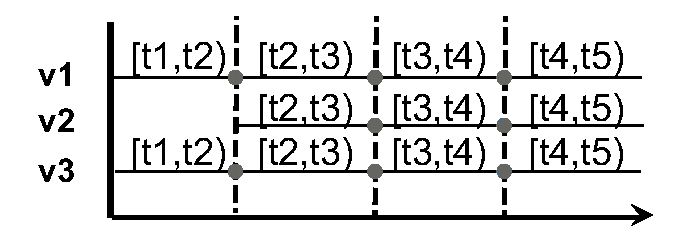
\includegraphics[width=1.6in]{figs/split.pdf}
\caption{with fragments}
\vspace{-0.2cm}
\label{fig:split}
\end{subfigure}
\begin{subfigure}[b]{1.6in}
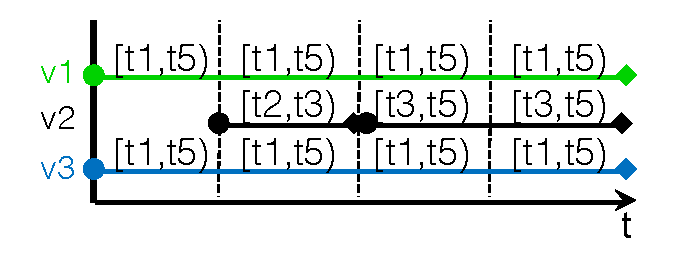
\includegraphics[width=1.6in]{figs/split2.pdf}
\caption{with full timestamps}
\vspace{-0.2cm}
\label{fig:split2}
\end{subfigure}
%\caption{Relation V from Figure~\ref{fig:coalesced} split in 4 partitions.}
\caption{Vertices from Figure~\ref{fig:snapshots} split in 4 partitions.}
\vspace{-0.5cm}
\end{figure}

{\bf Snapshot reducibility.}  Evolving graphs can be partitioned among
the available machines using time locality.  Following convention, we
refer to the operator that can produce such partitioning as a {\em
  splitter}.  The splitter places each tuple (vertex or edge) into one
or more partitions based on its timestamp.  The goal of the splitter
is to form partitions that are balanced, i.e., have approximately the
same number of items, under the assumption that most operations can be
executed locally at each partition.  Recall that snapshot reducibility
requires a temporal operator to produce the same result as if it were
evaluated over each snapshot.  Validity period of a tuple that spans
more than one temporal partition is split, and the tuple is replicated
across partitions.  This increases the overall size of the relation,
but all operations can now be carried out within each partition.  See
Figure~\ref{fig:split} for a simple example of the $V$ relation being
split into four temporal partitions.  

For the purposes of illustration, consider the temporal subgraph
operation, a generalization of subgraph matching for non-temporal
graphs~\cite{PortalarXiv2016}.  Temporal vertex-subgraph
\subv{q^t_v}{\ttt} computes an induced subgraph of \tve $\tve'(\tv',
\te', \tav', \tae')$, with vertices defined by the temporal
conjunctive query $q^t_v$.  Note that this is a subgraph query, and so
$\tv' \subseteq^T \tv$.  Observe that we can carry out the subgraph
operation with non-temporal predicates, e.g., \insql{name='Alice'}, at
each partition individually, without any cross-partition
communication.

The question of optimal splitting has been addressed by Le et
al.~\cite{Le2013}, who demonstrated that a temporal relation can be
efficiently split into $k$ buckets in cases of both internal memory
and external memory and guarantee optimality of solution\eat{in $O(N
  log N)$ time in internal memory and in $O(SORT(N)$ I/Os in external
  memory}.  This method requires a sequential scan of the relation to
compute an index called the stabbing count array.  How to make this
method more efficient in a distributed environment is an open
question.

\eat{ However, Le's approach is not the most efficient in a
distributed environment because it requires a sequential scan of the
relation to compute the stabbing array.  We have found an approach
that is parallelizable (no sequential scan) and completes in $O(N*m)$
time, where $N$ is the size of the relation and $m$ is the number of
distinct starting values.  In typical evolving graphs this $m$ is
significantly smaller than $log n$ and is thus faster than Le's
approach with and without parallelization.}

A number of alternatives for co-partitioning of graph relations
present themselves, as the vertex, edge and attribute relations are
not guaranteed to have the same splitters due to different evolution
rates.  Typically, vertices are co-partitioned with edges in the
non-temporal case~\cite{DBLP:conf/osdi/GonzalezXDCFS14}, and this
likely is most efficient with evolving graphs as well.  The subgraph
operation requires such co-partitioning to enforce referential
integrity on edges.

\eat{
Temporal partitioning is also appropriate for binary operators as long
as the two input relations are partitioned together, i.e., have the
same splitters.}  
\eat{Because each entity (vertex or edge) evolves at
  a different rate, the boundaries of partitions will require
  splitting of some of the tuples such that they reside in more than
  one partition.}  
\eat{An open question is what to do when a binary
operator is applied to two relations that are already partitioned
independently -- it may be more efficient to repartition one of them
using the splitters of the other, or apply the operator over existing
partitions and accept the cost of cross-partition communication.}

\eat{{\bf Temporal partitioning.}  In temporal algebra with point
semantics all queries can be carried out independently at each time
partition, which means that the cross-partition communication is not
necessary.  }

\eat{As long as the full timestamp is
preserved in each fragment after the split, both the snapshot
reducibility and extended snapshot reducibility properties are
observed using the approach in~\cite{Dignos2012}.}  

{\bf Extended snapshot reducibility.}  Snapshot reducibility can be
guaranteed in the distributed setting, as shown above.  \eat{Extended
  snapshot reducibility and change preservation require additional
  work.  }Subgraph query $q^t_v$ may use any of the constituent
relations of \tve, and may explicitly reference temporal information
in compliance with the extended snapshot reducibility property of
sequenced semantics.  Refer back to Figure~\ref{fig:split} and assume
time granularity of years.  If we perform the subgraph operation,
selecting vertices that persist for longer than 2 years, over the
split then we will get no matches.  However, the original relation
contains two matches -- only Bob \eat{with \insql{vid=2} }does not
meet the predicate.  To support extended snapshot reducibility over a
split relation, during partitioning tuples should be placed into their
partitions with their full original timestamps.  Incidentally, this is
what Le at al. describe in their work on optimal
splitters~\cite{Le2013}.  Figure~\ref{fig:split2} shows relation $V$
split in the same four partitions with this approach.

{\bf Change preservation.}  Change preservation property requires that
derived tuples should only be coalesced if they share lineage.  To
support this property, normalize and align operators are
used~\cite{Dignos2012}.  The normalize operator splits each tuple in
the input relation w.r.t. a group of tuples such that each timestamp
fragment is either fully contained or disjoint with every timestamp in
the group.  The align operator splits each tuple w.r.t. a group of
tuples such that each timestamp fragment is either an intersection
with one of the tuples in the group or is not covered by any tuple in
a group.\eat{ (See Figure 2 in~\cite{Dignos2012} for an
  illustration.)}

The normalize operator splits each tuple w.r.t. to a group defined by
the operation.  For example, consider attribute-based node creation
operation on graphs~\cite{PortalarXiv2016}, an operation similar to
aggregation on temporal relations.  This operation allows the user to
generate a \tg in which vertices correspond to disjoint groups of
vertices in the input that agree on the values of all grouping
attributes.  For instance, $\insql{node}^T_a(school,\tve)$ will
compute a vertex for each value of $\tav.a.school$.  While the group
defined for each tuple (distinct value of $school$) spans temporal
partitions, only tuples within the same partitions overlap.  Thus the
normalize operation can be carried out at each partition locally.
Similarly for the align operator.

An important challenge to address is how to efficiently support
aggregation over temporal windows in the distributed setting.  This
operation requires cross-partition communication, which impacts the
cost model, and was not considered in Le et al.~\cite{Le2013}.

{\bf Spatio-temporal partitioning.}  Large evolving graphs present
additional challenges compared to static graphs and temporal relations
alone.  Each graph snapshot may be too large to fit into a single
partition.  This necessitates partitioning graphs by both time and
structure.  Miao et al.~\cite{Miao2015} have demonstrated within their
ImmortalGraph system that different locality, structural or temporal,
is more appropriate for different graph queries.  However, the results
do not directly translate into the distributed environment because of
the parallelism gains.  While Miao et al. showed that spatial locality
provides better performance than temporal locality in global-point
queries, i.e., queries that compute something over a snapshot for a
particular time point.  In a distributed setting we do not expect
these results to hold since the communication costs generally dominate
the overall performance, and partitioning by time alone will guarantee
that a snapshot is distributed among the lowest number of partitions.

Global range queries such as change in graph centrality over time, on
the other hand, are computed over multiple snapshots and their
performance depends on the method of computation.  We can utilize
temporal locality and compute each snapshot independently.  Assuming
that each partition fits one or more snapshots, the maximum number of
snapshots across all partitions will determine the overall
performance.  With structural locality we can distribute edges across
the partitions using any of the already proposed partitioning
approaches such as range- and hash-based~\cite{Seo2013} or the
EdgePartition2D (E2D).  \eat{In E2D, a sparse edge adjacency matrix is
partitioned in two dimensions, guaranteeing a $2 \sqrt{n}$ bound on
vertex replication, where $n$ is the number of partitions. E2D has
been shown to provide good performance for Pregel-style
analytics~\cite{DBLP:conf/osdi/GonzalezXDCFS14}.  To minimize
communication with this partition approach caused by the time
dimension, we can use a batching method, effectively computing the
query over all snapshots simultaneously.  }

We explored the effectiveness of partitioning strategies in graphs
that undergo changed in topology over time, and found that structural
partitioning such as in ImmortalGraph is effective only when graph
topology changes very little~\cite{MoffittTempWeb16}.  We found that a
hybrid approach that combines temporal and structural locality is
promising.  \eat{ even with sub-optimal temporal partitioning.  In the
  hybrid approach, graphs are distributed first temporally and then
  the batching method is used within each partition.  Alternatively,
  if graphs are too large to fit into a single partition, partitions
  are divided into $k$ buckets, where $k$ is a divisor of the total
  number of partitions.  Then E2D strategy is used to partition the
  edges within the bucket among the partitions of that bucket.}  We
are currently investigating methods for selecting the spatio-temporal
partitioning strategy that provides the best overall performance.

\begin{table}
\centering
\caption{Connected components and PageRank with different temporal partitioning, seconds.}
\vspace{-0.2cm}
\begin{subtable}{0.229\textwidth}
\small
\caption{wiki-talk}
\vspace{-0.2cm}
\begin{tabular}{| l | c | c | c |}
\hline
\multicolumn{1}{|l|}{\bfseries width} & \multicolumn{1}{c|}{\bfseries k} & \multicolumn{1}{c|}{\bfseries CC} & \multicolumn{1}{c|}{\bfseries PR} \\ \hline
8 & 23 & 382 & 1,086 \\ \hline
16 & 12 & 328 & 1,037 \\ \hline
bal. & 16 & 351 & 720 \\ \hline
bal. & 24 & 408 & 375 \\ \hline
\end{tabular}
\label{fig:splitwiki}
\end{subtable}
\begin{subtable}{0.229\textwidth}
\small
\caption{nGrams}
\vspace{-0.2cm}
\begin{tabular}{| l | c | c | c |}
\hline
\multicolumn{1}{|l|}{\bfseries width} & \multicolumn{1}{c|}{\bfseries k} & \multicolumn{1}{c|}{\bfseries CC} & \multicolumn{1}{c|}{\bfseries PR} \\ \hline
8 & 26 & 1,324 & 2,867 \\ \hline
16 & 13 & 856 & 1,873  \\ \hline
bal. & 3 & 321 & 740  \\ \hline
bal. & 16 & 422 & 519 \\ \hline
\end{tabular}
\label{fig:splitngrams}
\end{subtable}
\label{tab:splitres}
\vspace{-0.4cm}
\end{table}

%\begin{figure*}
%\begin{subfigure}{0.45\textwidth}
%\includegraphics[width=3.4in]{figs/splitters_wiki.pdf}
%\label{fig:splitwiki}
%\caption{wiki-talk}
%\end{subfigure}
%\begin{subfigure}{0.45\textwidth}
%\includegraphics[width=3.4in]{figs/splitters_ngrams.pdf}
%\label{fig:splitngrams}
%\caption{nGrams}
%\end{subfigure}
%\caption[]{Connected components and PageRank with different temporal partitioning.}
%\label{fig:splitres}
%\end{figure*}

{\bf Preliminary experiments.}  We conducted some preliminary
experiments to see the effect of temporal partitioning on distributed
execution of analytics, which present one of the heaviest
computational workloads.  PageRank and Connected components analytics
were executed on the wiki-talk\footnote{\url{http://dx.doi.org/10.5281/zenodo.49561}} and nGrams\footnote{\url{http://storage.googleapis.com/books/ngrams/books/datasetsv2.html}}
datasets.

Wiki-talk contains 179 time periods.  nGrams contains over 400, but we
used the first 208.  Both datasets exhibit strong skew, with few edges
at the start of the datasets and increasing by several orders of
magnitude towards the end.  We compared equi-width and equi-depth
temporal partitioning, using 8 and 16 consecutive intervals for
equi-width, and using offline optimal split of edges with varying
number of splitters $k$.  Each dataset was partitioned first
temporally, and then spatially using Edge2D partitioning.
Table~\ref{tab:splitres} shows that equi-depth partitioning is
superior to equi-width in all but one cases.  However, the number of
splitters is key in obtaining good results.  We are currently
investigating this phenomenon further.
